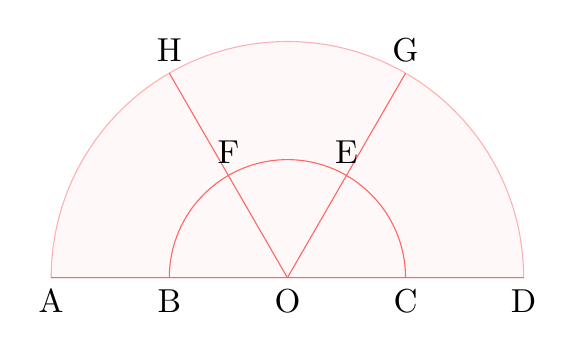
\begin{tikzpicture}	
  
    
\def \CharSize {1.2};
\def \BulletSize {1};


    %Définition de l 'angle de rotation de la figure
    \def \Rotation {0} 
    %Couleur des élèments de la figure (sauf le remplissage)
    \def \RapColor {red!60}


\begin{scope}[rotate=\Rotation]
    % contours
    \draw[color=\RapColor, fill =red!5, opacity=0.5] (-3,0) arc(180:0:3)--(3,0)--(-3,0)--cycle;	%Dont couleur de remplissage
    \draw[color=\RapColor] (-3,0)--(3,0);
    
   % demi-cercle intérieur :
    \draw[color=\RapColor](-1.5,0) arc(180:0:1.5);
    
    % rayons :
   \foreach \a in {0,60,...,180}{\draw[color=\RapColor] (\a:3)--(\a:0);}
   
 
  
\end{scope}

\draw (0,0) node [below,scale=\CharSize]{O};
\draw (1.5,0) node [below,scale=\CharSize]{C};
\draw (3,0) node [below,scale=\CharSize]{D};
\draw (-1.5,0) node [below,scale=\CharSize]{B};
\draw (-3,0) node [below,scale=\CharSize]{A};
\draw (60:1.5) node [above,scale=\CharSize]{E};
\draw (120:1.5) node [above,scale=\CharSize]{F};
\draw (60:3) node [above,scale=\CharSize]{G};
\draw (120:3) node [above,scale=\CharSize]{H};
    
\end{tikzpicture} 
